\documentclass[11pt,a4paper]{article}

% ---------- standard packages, black text only ----------
\usepackage[margin=2.5cm]{geometry}
\usepackage[T1]{fontenc}
\usepackage[utf8]{inputenc}
\usepackage{amsmath}
\usepackage{booktabs}
\usepackage{graphicx}
\usepackage{float}
\usepackage{enumitem}
\usepackage{tikz}
\usetikzlibrary{positioning,arrows.meta}
\usepackage[hidelinks]{hyperref}
\setlength{\parindent}{0pt}
\setlength{\parskip}{6pt}
\setlength{\emergencystretch}{3em}
\setlist{itemsep=2pt,topsep=3pt}

% file names in typewriter font
\newcommand{\file}[1]{\texttt{#1}}

% figure helper: shows the picture if the figures folder was uploaded, a plain box if not
\newcommand{\fig}[3]{%
  \begin{figure}[H]\centering
  \IfFileExists{figures/#1}{\includegraphics[width=#2\linewidth]{figures/#1}}{%
  \IfFileExists{../figures/#1}{\includegraphics[width=#2\linewidth]{../figures/#1}}{%
  \fbox{\parbox{0.8\linewidth}{\centering Figure file \texttt{\detokenize{#1}} not found.\\
  Put the \texttt{figures} folder next to this file (Overleaf) or keep this file in \texttt{docs/} of the repository.}}}}
  \caption{#3}
  \end{figure}}

\title{Plane-Wave Ultrasound Imaging Chain Simulation\\[2pt]
\large Project Explanation for the Team}
\author{Final Project -- Ultrasound Transducer and Beamforming Design\\
Simulator: MUST (Python version \texttt{pymust})}
\date{}

\begin{document}
\maketitle
\tableofcontents
\newpage

% =====================================================================
\section{Project description}
% =====================================================================

\subsection{The idea in one paragraph}
An ultrasound machine sends a short sound pulse into the body, listens for the echoes, and turns the echoes into a grey picture. Many things affect the picture: the shape of the probe, the pulse, how the wave is sent, how tissue scatters it, and how the echoes are combined. A real machine is costly and hides these steps. In this project we build \emph{every step in software}, in one chain, so we can plot and measure each step.

\subsection{What we simulate}
\begin{center}
\begin{tabular}{@{}p{4.0cm}p{10.5cm}@{}}
\toprule
\textbf{Part} & \textbf{Our choice}\\
\midrule
Probe & Linear array, 128 elements, pitch 0.3048 mm, element width 0.2698 mm (like an L9-4/38)\\
Pulse & Centre frequency 5 MHz, bandwidth about 3--7 MHz\\
Sampling and speed & Sampling 80 MHz, speed of sound 1540 m/s\\
Transmit & Plane wave at $0^\circ$, or 21 angles from $-20^\circ$ to $+20^\circ$ (compounding)\\
Targets & A single point, wires (with a close pair), and a speckle background with two cysts\\
Receive & 32-element sub-aperture (9.75 mm) on every scan line\\
Beamforming & Our own delay-and-sum (DAS) code that accepts any weights\\
Image & Envelope, normalize, log compression, 60 dB display (40 dB for the close pair)\\
Optional extra & Null Subtraction Imaging (NSI) from the reference paper, applied to the same data\\
\bottomrule
\end{tabular}
\end{center}

\subsection{Rules of the project}
\begin{itemize}
\item The main deliverable is the \emph{complete simulated imaging chain}.
\item NSI is optional. It is a second beamformer that we compare with normal DAS.
\item Artifacts (speckle, clutter, NSI side effects) are \emph{shown and explained, not fixed}.
\item All methods use the \emph{same saved RF data}, so the comparison is fair.
\end{itemize}

\subsection{Reference paper}
A.~Agarwal, J.~Reeg, A.~S.~Podkowa, M.~L.~Oelze, ``Improving spatial resolution using incoherent subtraction of receive beams having different apodizations,'' \emph{IEEE Trans.\ Ultrason.\ Ferroelectr.\ Freq.\ Control}, vol.~66, no.~1, pp.~5--17, 2019.

% =====================================================================
\section{Simplified physics}
% =====================================================================

\subsection{Sound in tissue}
Ultrasound is a pressure wave at a frequency above what we hear (medical imaging uses about 2--15 MHz). In soft tissue it travels at about $c = 1540$ m/s. The wavelength is
\begin{equation}
\lambda = \frac{c}{f}\qquad\Rightarrow\qquad \lambda \approx 0.31\ \text{mm at 5 MHz.}
\end{equation}
The wave bounces back where the tissue changes. At the border of two materials with acoustic impedances $Z_1$ and $Z_2$, the share of the wave that returns is
\begin{equation}
R = \frac{Z_2 - Z_1}{Z_2 + Z_1}.
\end{equation}

\subsection{Depth from time}
The probe sends a pulse and waits for the echo. The sound goes down and comes back, so the distance is travelled twice:
\begin{equation}
z = \frac{c\,t}{2}.
\end{equation}
Example: an echo that arrives after 24.7 $\mu$s comes from $z = 1540\times 24.7\times10^{-6}/2 \approx 19$ mm.

\subsection{Scattering and speckle}
Tissue holds many tiny scatterers, much smaller than the wavelength. Each one sends back a weak echo. The signal from one small region is the sum of many echoes with random phases. This makes the grainy pattern called \textbf{speckle}.
\begin{itemize}
\item A \textbf{wire} or \textbf{point} is one strong scatterer.
\item The \textbf{tissue background} is thousands of weak random scatterers.
\item An \textbf{anechoic cyst} has no scatterers inside (strength 0), so it should look dark.
\item A \textbf{hyperechoic cyst} has stronger scatterers than the background (we use $\times 4$, about $+12$ dB), so it should look bright.
\end{itemize}
For fully developed speckle the envelope follows a Rayleigh distribution, and its speckle SNR (mean divided by standard deviation) is about \textbf{1.91}. Lower values mean the speckle is ``under-developed''.

\subsection{The probe and the pulse}
Each element is a piezoelectric crystal. It turns an electrical pulse into pressure, and turns the returning echo back into a voltage. Our array has $N = 128$ elements, spaced by the pitch $d = 0.3048$ mm (about one wavelength at 5 MHz). A short pulse has a wide bandwidth $B$, and the depth detail (axial resolution) is roughly $c/(2B)$.

The ideal pulse is a Gaussian-shaped sine wave:
\begin{equation}
s(t) = e^{-t^2/(2\sigma^2)}\cos(2\pi f_0 t),\qquad f_0 = 5\ \text{MHz}.
\end{equation}

\subsection{Plane-wave transmission}
In plane-wave imaging, all elements fire together. One transmission lights up the whole image, so the frame rate is very high. To tilt the wave by an angle $\theta$, element $i$ at position $x_i$ fires with a delay
\begin{equation}
\tau_i(\theta) = \frac{x_i\sin\theta}{c}
\end{equation}
(plus a constant so that no delay is negative). The wave front reaches a point $(x,z)$ at time
\begin{equation}
t_{tx}(x,z) = \frac{x\sin\theta + z\cos\theta}{c} + t_{\text{off}}.
\end{equation}
Here $t_{\text{off}}$ is the constant shift: the first element to fire defines $t=0$. One plane wave gives a lower-quality image than a focused beam. \textbf{Compounding} fixes this: send several angles, beamform each, and \emph{add the RF images before the envelope}.

\subsection{Receive beamforming: delay and sum (DAS)}
The echo from pixel $(x,z)$ reaches element $i$ after
\begin{equation}
t_{rx,i}(x,z) = \frac{\sqrt{(x-x_i)^2 + z^2}}{c}.
\end{equation}
DAS reads each channel at the right time and adds them with weights $w_i$ (the \emph{apodization}):
\begin{equation}
y(x,z) = \sum_{i} w_i\; s_i\!\big(t_{tx}(x,z) + t_{rx,i}(x,z)\big).
\end{equation}
Why it works: if a real scatterer is at the pixel, all channel values line up and add up to a big number. If there is nothing there, they do not line up and they cancel.

We use a 32-element sub-aperture of width $D = 32\times0.3048 \approx 9.75$ mm. The f-number is $F_\# = z/D$. At $z = 19$ mm, $F_\# \approx 1.95$.

\subsection{Beam shape, resolution and apodization}
The beam of an aperture has a main lobe and side lobes (like a window in signal processing). With equal weights, the first side lobe is about $-13$ dB. The side-to-side (lateral) detail is set by the main lobe width:
\begin{equation}
\Delta x \approx 1.41\,\lambda\,F_\# \qquad(\approx 0.85\ \text{mm at 19 mm depth}).
\end{equation}
Changing the weights (apodization) lowers side lobes but widens the main lobe. This \emph{resolution versus side lobe} trade-off is the main compromise in receive beamforming.

\subsection{From RF to a picture}
The beamformed RF signal wiggles at 5 MHz, but the picture shows its strength. The \textbf{envelope} is the size of the analytic signal (built with the Hilbert transform $\mathcal{H}$):
\begin{equation}
E = \left| y + j\,\mathcal{H}\{y\} \right|.
\end{equation}
Echoes differ greatly in strength, so we normalize and use a log scale (dynamic range 60 dB):
\begin{equation}
E_{\text{dB}} = 20\log_{10}(E) - \max\big(20\log_{10}(E)\big).
\end{equation}
Values below $-60$ dB are shown as black. The result is the \textbf{B-mode image}.

\subsection{Null Subtraction Imaging (optional)}
NSI uses three weight sets on the 32 elements:
\begin{itemize}
\item ZM (zero-mean): $+1$ on the first 16 elements, $-1$ on the last 16. Its beam has a \emph{null} (a dip to zero) straight ahead.
\item DC1 $=$ ZM $+\,c$, with a small constant $c$ (we test 0.01, 0.03, 0.05).
\item DC2 $=$ DC1 mirrored left to right.
\end{itemize}
We beamform the same RF data three times and subtract the envelopes:
\begin{equation}
E_{\text{NSI}} = \frac{E_{DC1}+E_{DC2}}{2} - E_{ZM}.
\end{equation}
Only the small ``bridge'' at the null survives, which leaves a \emph{very narrow peak}. A smaller $c$ gives a narrower peak. The price is a weaker peak and changed speckle, because subtracting envelopes is non-linear.

% =====================================================================
\section{Simulation workflow}
% =====================================================================

\subsection{The chain}
Figure~\ref{fig:chain} shows the order of the steps. The three steps in the first row are done by MUST. The rest is our own code.

\begin{figure}[H]\centering
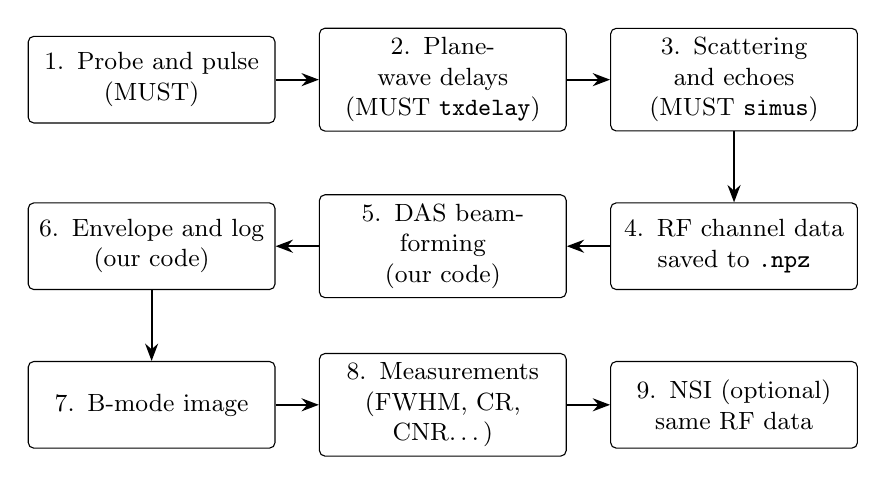
\begin{tikzpicture}[
  box/.style={draw,rectangle,rounded corners=2pt,minimum height=1.1cm,text width=2.9cm,align=center,font=\small},
  arr/.style={-{Stealth[length=2.2mm]},thick},
  node distance=0.55cm]
\node[box] (a) {1. Probe and pulse\\(MUST)};
\node[box,right=of a] (b) {2. Plane-wave delays\\(MUST \texttt{txdelay})};
\node[box,right=of b] (c) {3. Scattering and echoes\\(MUST \texttt{simus})};
\node[box,below=0.9cm of c] (d) {4. RF channel data\\saved to \texttt{.npz}};
\node[box,left=of d] (e) {5. DAS beamforming\\(our code)};
\node[box,left=of e] (f) {6. Envelope and log\\(our code)};
\node[box,below=0.9cm of f] (g) {7. B-mode image};
\node[box,right=of g] (h) {8. Measurements\\(FWHM, CR, CNR\ldots)};
\node[box,right=of h] (i) {9. NSI (optional)\\same RF data};
\draw[arr] (a)--(b); \draw[arr] (b)--(c); \draw[arr] (c)--(d);
\draw[arr] (d)--(e); \draw[arr] (e)--(f); \draw[arr] (f)--(g);
\draw[arr] (g)--(h); \draw[arr] (h)--(i);
\end{tikzpicture}
\caption{The simulated imaging chain, from probe to measurements.}\label{fig:chain}
\end{figure}

\subsection{Step by step}
\begin{enumerate}[label=\textbf{Step \arabic*.},leftmargin=*,labelsep=0.5em]
\item \textbf{Probe and pulse.} \file{config.py} (in \file{src/lib}) holds the numbers. The function \texttt{make\_param()} builds the MUST probe: 128 elements, pitch, width, 5 MHz, 80\% bandwidth, 80 MHz sampling.
\item \textbf{Plane-wave delays.} MUST function \texttt{txdelay} gives the firing delay of every element for a chosen angle. At $0^\circ$, all delays are zero.
\item \textbf{Scattering.} MUST function \texttt{simus} takes the scatterer list $(x, z, \text{strength})$ and the delays. It adds the echoes of all scatterers at all 128 elements.
\item \textbf{RF data.} The output is a table \emph{time $\times$ 128 elements} for each angle. We save it as \texttt{rf[angle, time, channel]}. Optional white noise at 35 dB or 10 dB SNR is added to a copy.
\item \textbf{DAS beamforming.} For every pixel, our code computes $t_{tx} + t_{rx,i}$ for the 32 elements, reads the RF at that time (linear interpolation), multiplies by the weights and adds.
\item \textbf{Compounding.} For several angles, the RF images are added \emph{before} the envelope. This keeps the phase.
\item \textbf{Image formation.} Envelope, normalize, log, clip at $-60$ dB (or $-40$ dB for the close pair).
\item \textbf{Measurements.} Beam widths, side lobes, contrast ratio, CNR, speckle SNR (formulas below).
\item \textbf{NSI (optional).} Same RF data, three weight sets, subtract the envelopes.
\end{enumerate}

\subsection{The measurements}
\begin{itemize}
\item \textbf{FWHM} (full width at $-6$ dB): the width of the beam where it falls to half amplitude. Smaller is better. We measure it sideways (lateral) and along depth (axial).
\item \textbf{Peak side lobe:} the strongest level outside the main lobe. Lower is better.
\item \textbf{Contrast ratio:} $\mathrm{CR} = 20\log_{10}(\mu_{\text{in}}/\mu_{\text{bg}})$, with the mean envelope inside a cyst and in the background around it.
\item \textbf{Contrast-to-noise ratio:} $\mathrm{CNR} = |\mu_{\text{in}}-\mu_{\text{bg}}|/\sqrt{\sigma_{\text{in}}^2+\sigma_{\text{bg}}^2}$.
\item \textbf{Speckle SNR:} mean divided by standard deviation of the background envelope (about 1.91 for fully developed speckle). We average it over $3\times3$ mm blocks so slow brightness changes do not distort it.
\end{itemize}
The cyst region of interest is a disc of 0.8 of the cyst radius. The background is a ring from 1.3 to 1.9 radii around the cyst.

\subsection{The three phantoms}
\begin{center}
\begin{tabular}{@{}p{2.4cm}p{12.1cm}@{}}
\toprule
\textbf{Phantom} & \textbf{Content}\\
\midrule
Point & One scatterer at $x=0$, $z=19$ mm.\\
Wires & Three wires at $z = 10, 20, 30$ mm on the centre line; a close pair at $z=18$ mm, $x=\pm0.4$ mm (0.8 mm apart); plus a weak speckle background (4480 scatterers).\\
Contrast & Random scatterers for $x=\pm15$ mm, $z=10$--$40$ mm (40 per mm$^2$ at full density, about 14 per resolution cell). Anechoic cyst: centre $(-6, 20)$ mm, radius 4 mm, strength $\times0$. Hyperechoic cyst: centre $(+6, 30)$ mm, radius 4 mm, strength $\times4$.\\
\bottomrule
\end{tabular}
\end{center}

\subsection{What is not in the model}
\begin{itemize}
\item No tissue attenuation, so no depth-gain compensation is needed.
\item The simulation is 2-D by default (\texttt{USE\_3D = False}), so the 19 mm elevation focus is ignored.
\item Linear acoustics only (no harmonics or non-linear effects).
\end{itemize}

% =====================================================================
\section{What each file does}
% =====================================================================

\subsection{Folder structure}
\begin{verbatim}
simulating-US-imaging-chain/
  data/                 RF data (.npz, not in git) and metrics (.json)
  figures/              output pictures (.png)
  docs/                 this explanation (.tex) and the proposal (.pdf)
  src/
    lib/                library: an importable package called "lib"
      __init__.py
      config.py
      phantoms.py
      beamformer.py
      metrics.py
    scripts/            programs you run
      01_probe_pulse.py
      02_phantoms.py
      03_simulate.py
      04_das.py
      05_nsi.py
      06_validate.py
      run_all.py
  LICENSE
  README.md
  requirements.txt
  pyproject.toml
  .gitignore
\end{verbatim}
The idea: \file{src/lib} holds code that is \emph{imported}, \file{src/scripts} holds code that is \emph{run}. Scripts import the library with lines such as \texttt{from lib import config as cfg}.

\subsection{Library files (\file{src/lib})}
\begin{center}
\small
\begin{tabular}{@{}p{3.6cm}p{11.0cm}@{}}
\toprule
\textbf{File} & \textbf{What it does}\\
\midrule
\file{config.py} & Holds \emph{every} number (probe, angles, phantom sizes, dynamic range, NSI $c$) and builds the MUST probe. It also sets the paths of \file{data/} and \file{figures/} in the repository root. Change numbers only here.\\
\file{phantoms.py} & Builds the scatterer lists for the point, wire and contrast phantoms.\\
\file{beamformer.py} & Our DAS beamformer with any weights, angle compounding, envelope and log functions, and the NSI weights and image function.\\
\file{metrics.py} & The measurement functions: FWHM, peak side lobe, CR, CNR, speckle SNR.\\
\file{\_\_init\_\_.py} & Marks the folder as a Python package.\\
\bottomrule
\end{tabular}
\end{center}

\subsection{Script files (\file{src/scripts})}
\begin{center}
\small
\begin{tabular}{@{}p{3.6cm}p{11.0cm}@{}}
\toprule
\textbf{File} & \textbf{What it does}\\
\midrule
\file{01\_probe\_pulse.py} & Plots the array and the pulse (formula and simulated) with their spectra. Prints the $-6$ dB bands.\\
\file{02\_phantoms.py} & Plots the three scatterer maps and prints the scatterer counts.\\
\file{03\_simulate.py} & Runs MUST for each phantom and angle, cuts the useless late samples, optionally adds noise, and saves \file{data/*.npz}. Options: \texttt{-{}-quick}, \texttt{-{}-medium}, \texttt{-{}-noise}, \texttt{-{}-only}.\\
\file{04\_das.py} & Forms the normal DAS images, measures point, wires and cysts, and checks our beamformer against MUST's \texttt{dasmtx}. Writes \file{data/metrics\_04.json}.\\
\file{05\_nsi.py} & Does the same with NSI on the saved data and sweeps $c$. Writes \file{data/metrics\_05.json}.\\
\file{06\_validate.py} & The automatic test suite (39 checks, PASS or FAIL).\\
\file{run\_all.py} & Runs all six steps in order.\\
\bottomrule
\end{tabular}
\end{center}

\subsection{Other files}
\begin{center}
\small
\begin{tabular}{@{}p{3.6cm}p{11.0cm}@{}}
\toprule
\textbf{File} & \textbf{What it does}\\
\midrule
\file{README.md} & Overview, setup, run commands and expected outputs.\\
\file{LICENSE} & The MIT licence text.\\
\file{requirements.txt} & The Python packages: \texttt{pymust}, \texttt{numpy}, \texttt{scipy}, \texttt{matplotlib}.\\
\file{pyproject.toml} & Lets \texttt{pip install -e .} make the \texttt{lib} package importable.\\
\file{.gitignore} & Keeps the large \file{.npz} data files and temporary files out of git.\\
\file{docs/} & This explanation (\file{project\_explanation.tex}) and the project proposal.\\
\bottomrule
\end{tabular}
\end{center}

\subsection{Setup, run order and time}
Set up once, from the repository root:
\begin{verbatim}
pip install -r requirements.txt
pip install -e .
\end{verbatim}
Then run the steps in order, always from the repository root. Step 3 is the slow one:
\begin{center}
\small
\begin{tabular}{@{}p{7.4cm}p{3.6cm}p{3.1cm}@{}}
\toprule
\textbf{Command} & \textbf{Contrast phantom} & \textbf{Time (1 core)}\\
\midrule
\texttt{python src/scripts/03\_simulate.py -{}-quick} & 5 angles, half density & about 4 min\\
\texttt{python src/scripts/03\_simulate.py -{}-medium} & 21 angles, half density & about 15 min\\
\texttt{python src/scripts/03\_simulate.py} & 21 angles, full density & about 40 min\\
\bottomrule
\end{tabular}
\end{center}
Then run \file{04\_das.py}, \file{05\_nsi.py} and \file{06\_validate.py} the same way (for example \texttt{python src/scripts/04\_das.py}), or run everything with:
\begin{verbatim}
python src/scripts/run_all.py --quick --noise
\end{verbatim}
The results in this document come from the \textbf{21-angle, half-density} run (20 scatterers per mm$^2$).

\subsection{Data files in the \file{data} folder}
\begin{center}
\small
\begin{tabular}{@{}p{5.2cm}p{9.3cm}@{}}
\toprule
\textbf{File} & \textbf{Content}\\
\midrule
\file{point.npz}, \file{wires.npz}, \file{contrast.npz} & \texttt{rf[angle, time, channel]} (float32), the angles, sampling rate, scatterer positions and strengths. Time starts at 0 and is sampled at 80 MHz. For \file{contrast}: 21 angles, 5675 samples, 128 channels (about 61 MB).\\
\file{*\_snr35.npz}, \file{*\_snr10.npz} & The same data with noise added (35 dB and 10 dB SNR).\\
\file{metrics\_04.json} & All DAS measurements.\\
\file{metrics\_05.json} & All NSI measurements.\\
\bottomrule
\end{tabular}
\end{center}

% =====================================================================
\section{Results and validation}
% =====================================================================

\subsection{How we check the simulation}
We use four kinds of checks:
\begin{enumerate}
\item \textbf{Known positions:} a point at 19 mm must appear at 19 mm. Wires at 10, 20, 30 mm must appear there.
\item \textbf{Theory:} the beam width must match the formula, and the shape must match the sinc curve.
\item \textbf{Second opinion:} our DAS must match MUST's own \texttt{dasmtx} on the same data.
\item \textbf{Known truth:} the hyperechoic cyst was made $\times4$ stronger, so its contrast must be near $+12$ dB.
\end{enumerate}
The test suite \file{06\_validate.py} runs 39 checks and prints PASS or FAIL for each. \textbf{All 39 pass.}

\begin{center}
\small
\begin{tabular}{@{}p{1.0cm}p{9.6cm}p{3.0cm}@{}}
\toprule
\textbf{Test} & \textbf{What is checked} & \textbf{Checks}\\
\midrule
T1 & Array length, aperture width, wavelength & 3\\
T2 & Transmit time offset and point position at $-20^\circ, -10^\circ, 0^\circ, +10^\circ, +20^\circ$ & 15\\
T3 & Point: depth, position, lateral and axial FWHM, side lobe, match with MUST & 6\\
T4 & Wire depths (10, 20, 30 mm); the 0.8 mm pair is not resolved (expected) & 4\\
T5 & Noisy data (35 dB and 10 dB): the 20 mm wire is still found within $\pm0.1$ mm & 2\\
T6 & Contrast phantom: CR of both cysts, speckle SNR (1 angle and compounded) & 4\\
T7 & NSI: narrower beam, width grows with $c$, lower side lobes, lower speckle SNR and CNR & 5\\
\midrule
 & \textbf{Total} & \textbf{39}\\
\bottomrule
\end{tabular}
\end{center}
T2 is important: it proves that our transmit-time formula (including $t_{\text{off}}$) agrees with MUST for tilted waves.

\subsection{Point target (conventional DAS, $0^\circ$)}
\begin{center}
\begin{tabular}{@{}p{7.2cm}p{3.5cm}p{3.5cm}@{}}
\toprule
\textbf{Quantity} & \textbf{Measured} & \textbf{Reference}\\
\midrule
Peak depth & 19.003 mm & 19.000 mm (true)\\
Peak lateral position & $-0.009$ mm & 0 mm (true)\\
Lateral FWHM & 0.79 mm & 0.72 mm (sinc) to 0.85 mm (Eq.\ 1.41$\lambda F_\#$)\\
Axial FWHM (envelope) & 0.24 mm & about $c/(2B)\approx0.2$--0.3 mm\\
Peak side lobe & $-19.5$ dB & $-13$ dB (ideal rectangular, single frequency)\\
Difference to MUST \texttt{dasmtx} & 0.16 dB RMS & 0 dB\\
\bottomrule
\end{tabular}
\end{center}
The side lobe is lower than $-13$ dB because the pulse is broadband: the side lobes of different frequencies are in different places and smear out.

\subsection{Wires}
\begin{center}
\begin{tabular}{@{}p{7.2cm}p{3.5cm}p{3.5cm}@{}}
\toprule
\textbf{Quantity} & \textbf{Measured} & \textbf{True}\\
\midrule
Wire 1 depth & 10.004 mm & 10 mm\\
Wire 2 depth & 19.995 mm & 20 mm\\
Wire 3 depth & 30.005 mm & 30 mm\\
Lateral FWHM of the 20 mm wire & 0.83 mm & --\\
Close pair (0.8 mm apart): dip between the two & $-0.3$ dB & --\\
\bottomrule
\end{tabular}
\end{center}
The pair is \emph{not} resolved. This is expected: 0.8 mm is about the same as the lateral FWHM (0.79 mm), so the two echoes blend into one blob.

\subsection{Contrast phantom (conventional DAS)}
\begin{center}
\begin{tabular}{@{}p{6.0cm}p{3.1cm}p{3.1cm}@{}}
\toprule
\textbf{Quantity} & \textbf{1 angle ($0^\circ$)} & \textbf{21 angles}\\
\midrule
Hyperechoic cyst: CR (true $+12.0$ dB) & $+11.4$ dB & $+12.0$ dB\\
Hyperechoic cyst: CNR & 1.23 & 1.15\\
Anechoic cyst: CR & $-15.2$ dB & $-23.6$ dB\\
Anechoic cyst: CNR & 1.44 & 1.43\\
Speckle SNR (block average) & 1.74 & 1.51\\
\bottomrule
\end{tabular}
\end{center}

\subsection{NSI results}
\textbf{Point target} (lateral FWHM measured on a fine line grid, because the NSI peak is very thin):
\begin{center}
\begin{tabular}{@{}p{5.0cm}p{3.0cm}p{3.0cm}p{3.0cm}@{}}
\toprule
\textbf{Method} & \textbf{Lateral FWHM} & \textbf{Peak vs.\ DAS peak} & \textbf{Side lobe}\\
\midrule
Conventional DAS & 793 $\mu$m & 0 dB & $-19.5$ dB\\
NSI, $c = 0.01$ & 9 $\mu$m & $-41$ dB & about $-61$ dB\\
NSI, $c = 0.03$ & 21 $\mu$m & $-31$ dB & about $-58$ dB\\
NSI, $c = 0.05$ & 33 $\mu$m & $-26$ dB & about $-56$ dB\\
\bottomrule
\end{tabular}
\end{center}
The side lobe values were measured on a coarser line grid than the widths, so treat them as approximate.

\textbf{Contrast phantom} (21 angles):
\begin{center}
\begin{tabular}{@{}p{6.0cm}p{3.1cm}p{3.1cm}@{}}
\toprule
\textbf{Quantity} & \textbf{DAS} & \textbf{NSI ($c=0.03$)}\\
\midrule
Hyperechoic cyst: CR & $+12.0$ dB & $+12.8$ dB\\
Hyperechoic cyst: CNR & 1.15 & 0.34\\
Anechoic cyst: CR & $-23.6$ dB & $-28.9$ dB\\
Anechoic cyst: CNR & 1.43 & 0.43\\
Speckle SNR & 1.51 & 0.44\\
\bottomrule
\end{tabular}
\end{center}

\subsection{What the figures tell us}
\fig{fig01_array.png}{0.8}{\texttt{fig01\_array}: the 128 elements. The red dots mark one 32-element sub-aperture (9.75 mm).}
\textbf{Figure 2 (array).} The sub-aperture is only a quarter of the array. Each scan line uses a different group of 32 elements, centred on that line.

\fig{fig02_pulse_spectrum.png}{0.95}{\texttt{fig02\_pulse\_spectrum}: the formula pulse (top) and the real simulated pulse-echo (bottom), in time (left) and frequency (right).}
\textbf{Figure 3 (pulse).} The formula pulse is built for a $-6$ dB band of exactly 3.0--7.0 MHz ($\sigma = 93.7$ ns). The pulse that MUST really produces has a band of 3.0--6.47 MHz with its peak near \textbf{4 MHz}, not 5 MHz. The reason is the element response that MUST adds. This is a property of the simulated probe, not an error.

\fig{fig03_phantoms.png}{1.0}{\texttt{fig03\_phantoms}: the three phantoms. Red dots: point and wires. Blue circle: anechoic cyst. Red circle: hyperechoic cyst.}
\textbf{Figure 4 (phantoms).} Dot size follows scatterer strength. Zero-strength scatterers are not drawn, so the anechoic cyst looks empty. The plot title counts every scatterer, including the zero-strength ones inside the anechoic cyst.

\fig{fig04_channel_data.png}{0.5}{\texttt{fig04\_channel\_data}: raw echoes of the wire phantom, time against element.}
\textbf{Figure 5 (channel data).} Each wire makes a curved line. The curve is lowest at the element right above the wire and bends to later times at the sides, because the echo has a longer way to the side elements. This curve is exactly what DAS flattens: it reads each channel along the curve and adds.

\fig{fig05_point_psf.png}{1.0}{\texttt{fig05\_point\_psf}: image of the point, lateral profile (own DAS, MUST, sinc theory) and axial profile.}
\textbf{Figure 6 (point spread function).} The point is the ``smallest thing the system can show''. Its image is the system's blur. The lateral profile of our DAS lies on top of MUST's curve (0.16 dB difference) and follows the sinc theory in the main lobe. This is the strongest proof that our beamformer is correct.

\fig{fig06_wires.png}{1.0}{\texttt{fig06\_wires}: wire phantom (left, 60 dB), close pair (middle, 40 dB), profile across the pair (right).}
\textbf{Figure 7 (wires).} The three wires are at the right depths. The close pair is one blob: the system cannot separate two points that are closer than its lateral FWHM.

\fig{fig07_contrast.png}{0.95}{\texttt{fig07\_contrast}: contrast phantom with 1 angle (left) and 21 angles compounded (right).}
\textbf{Figure 8 (contrast).} Both cysts are visible in both images. With 21 angles, the anechoic cyst is clearly darker ($-15.2$ dB $\to$ $-23.6$ dB) and the speckle looks more even in all directions. With one angle there is faint horizontal banding. In the single-angle image the dark cyst is partly filled with clutter.

\fig{fig08_nsi_point.png}{0.95}{\texttt{fig08\_nsi\_point}: lateral profiles for DAS and NSI with $c = 0.01, 0.03, 0.05$ (left) and the NSI image of the point (right).}
\textbf{Figure 9 (NSI point).} NSI makes the beam about 40 times thinner at $c = 0.03$, with much lower side lobes, but the peak is about 31 dB weaker. The smaller the $c$, the thinner and weaker the peak. This is the trade-off.

\fig{fig09_nsi_pair.png}{1.0}{\texttt{fig09\_nsi\_pair}: close pair with DAS and NSI.}
\textbf{Figure 10 (NSI close pair).} NSI does \emph{not} separate the two wires. Even in a clean test with only these two wires, NSI shows one peak at the point halfway between them. The reason: the two wires are symmetric, their echoes in the zero-mean beam have opposite sign and cancel at the centre line, which looks like a null with a bridge. This is an artifact. As agreed in the proposal, we describe it and do not fix it.

\fig{fig10_nsi_contrast.png}{0.95}{\texttt{fig10\_nsi\_contrast}: contrast phantom with DAS (left) and NSI (right), 21 angles.}
\textbf{Figure 11 (NSI contrast).} NSI keeps the cysts but makes the speckle thin and weak: speckle SNR falls from 1.51 to 0.44 and CNR from 1.15 to 0.34. This matches the reference paper, which reports a narrower beam but lower contrast and under-developed speckle.

\subsection{Main conclusions}
\begin{enumerate}
\item The chain works end to end: every position and size agrees with theory, with MUST, and with the known truth in the phantoms.
\item \textbf{Our own DAS beamformer is correct}: it matches MUST's \texttt{dasmtx} to 0.16 dB and passes the transmit-time test at five angles.
\item Lateral FWHM is about 0.8 mm at 19 mm depth, as the theory predicts. Two points closer than this cannot be separated.
\item Compounding 21 angles gives a darker anechoic cyst and more even speckle.
\item NSI gives a much thinner beam and lower side lobes, but weaker signal, lower CNR and thin speckle. It also creates a false peak between two close, symmetric wires.
\end{enumerate}

\subsection{Limits and notes}
\begin{itemize}
\item The data in this document is from \textbf{half the scatterer density} of the project plan (20 instead of 40 per mm$^2$, about 7 instead of 14 per resolution cell). The speckle SNR (1.51 to 1.74) is below 1.91 for this reason. Compounding makes the beam narrower, so fewer scatterers fall in each cell, which lowers the value further. A full-density run is needed to check whether the value moves closer to 1.91. We have not run it.
\item Compounding with only 5 angles hardly changed the contrast. Full benefit shows with many angles.
\item Noisy data (35 dB and 10 dB SNR) was saved and only tested for locating the 20 mm wire. We expect NSI to suffer most from noise because its peak is very weak. This is a good extra experiment.
\item The simulation is 2-D and has no attenuation.
\end{itemize}

% =====================================================================
\section{Short glossary}
% =====================================================================
\begin{center}
\small
\begin{tabular}{@{}p{3.3cm}p{11.2cm}@{}}
\toprule
\textbf{Term} & \textbf{Meaning}\\
\midrule
RF data & The raw voltage signals from the elements, before any image is made.\\
B-mode image & The grey picture made from the envelope of beamformed RF data.\\
Scatterer & A tiny point that sends back an echo.\\
Speckle & The grainy pattern from the random sum of many echoes.\\
Apodization & The weights $w_i$ applied to the channels before adding.\\
Aperture & The group of elements used to make one scan line (here 32).\\
DAS & Delay and sum: shift each channel in time, then add.\\
Compounding & Adding the images from several transmit angles.\\
FWHM & Width of a beam at half amplitude ($-6$ dB).\\
Side lobe & A weaker beam peak next to the main one; it causes haze.\\
CR, CNR & Contrast ratio and contrast-to-noise ratio (formulas in Section 3).\\
NSI & Null Subtraction Imaging: subtracting envelopes to get a very thin beam.\\
\bottomrule
\end{tabular}
\end{center}

\end{document}
